We report on the application of our method for surveillance synthesis in two case studies. We have implemented the simulation in \texttt{Python}, using the \texttt{slugs} reactive synthesis tool~\cite{EhlersR16}. The experiments were performed on an Intel i5-5300U 2.30 GHz CPU with 8 GB of RAM. In both cases, the target is being controlled by a human while the agent responds using the synthesized surveillance strategy.

\subsection{Liveness Surveillance Specification + Task Specification}
Figure~\ref{fig:case1} shows a gridworld divided into  regions. The surveillance objective requires the agent to infinitely often know precisely the location of the target (either see it, or have a belief consisting of one cell). Additionally, it has to perform the task of patrolling (visiting infinitely often) the green 'goal' cell. Formally, the specification is $\LTLglobally\LTLfinally p_1 \wedge \LTLglobally\LTLfinally \mathit{goal}$. The agent can move up to 3 grid cells away at each step. The sensor mode, that is, the visibility function, used here is 'line-of-sight' with a range of 5 cells. The agent cannot see through obstacles (shown in red) and cannot see farther than 5 cells away. 


\begin{figure}
\subfloat[Gridworld with a user provided abstraction partition with 7 sets, marked by black lines.. \label{fig:case1}]{
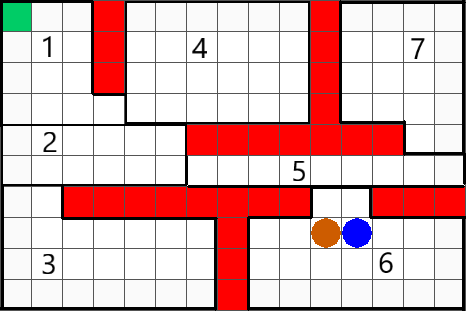
\includegraphics[scale=0.3]{figs/Liveness_part.png}
}
\hfill
\subfloat[Gridworld showing visibility of the agent. All locations shown in black are invisible to the agent. \label{fig:case1vis}]{
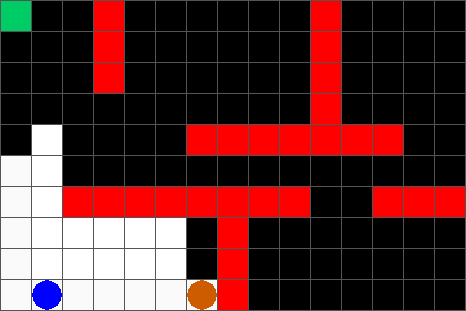
\includegraphics[scale=0.3]{figs/Liveness_t1.png}\hspace{.5cm}
}

\caption{10x15 gridworld with a surveillance liveness specification. The agent is blue, and the target to be surveilled is orange. Red states are obstacles.}
\label{fig:casestudies}

\end{figure}



Using the abstraction partition of size 7 shown in Figure \ref{fig:case1}, the overall number of states in the two-player game is $15\times10 + 2^7 = 278$ states. In contrast, solving the full abstract game will have in the order of $2^{150}$ states, which is a state-space size that state-of-the-art synthesis tools cannot handle. 

\begin{figure}
\begin{minipage}{5.0cm}
	\centering
		\subfloat[$t_1$ \label{fig:case1t2}]{
		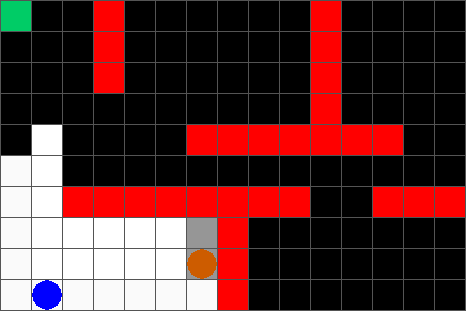
\includegraphics[scale=0.17]{figs/Liveness_t2.png}\hspace{.5cm}
	}
	\subfloat[$t_3$ \label{fig:case1t3}]{
		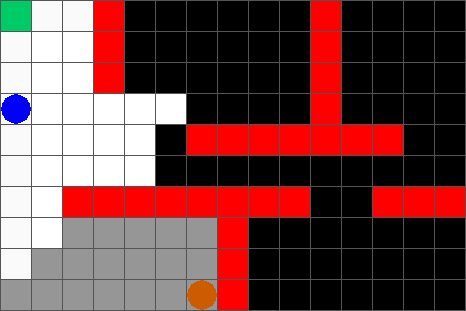
\includegraphics[scale=0.17]{figs/Liveness_t3.png}\hspace{.5cm}
	}
	\subfloat[$t_4$ \label{fig:case1t4}]{
	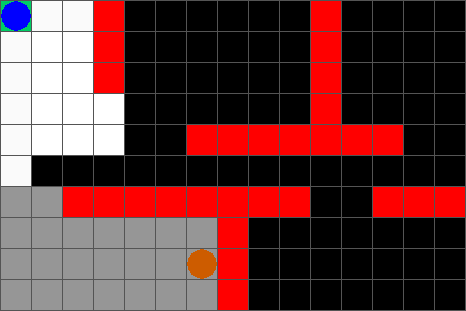
\includegraphics[scale=0.17]{figs/Liveness_t4.png}\hspace{.5cm}
}
\end{minipage}
\begin{minipage}{5.0cm}
	\centering
	\subfloat[$t_5$  \label{fig:case1t5}]{
		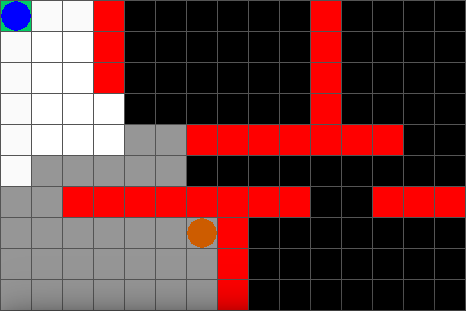
\includegraphics[scale=0.17]{figs/Liveness_t5.png}\hspace{.5cm}
	}
	\subfloat[$t_6$ \label{fig:case1t6}]{
		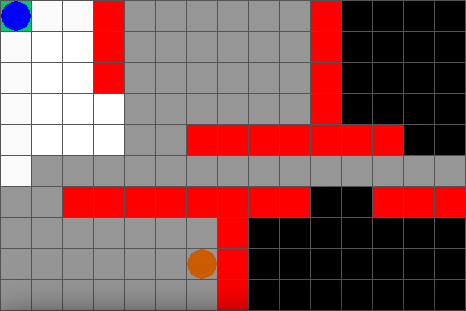
\includegraphics[scale=0.17]{figs/Liveness_t6.png}\hspace{.5cm}
	}
	\subfloat[$t_7$ \label{fig:case1t7}]{
		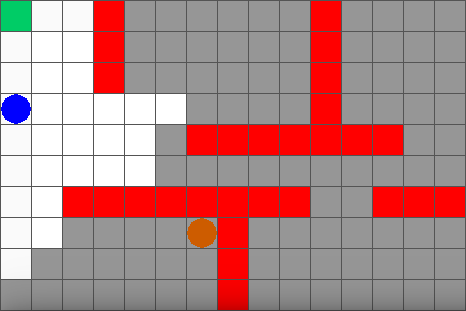
\includegraphics[scale=0.17]{figs/Liveness_t7.png}\hspace{.5cm}
	}
	
\end{minipage}

	
	\caption{Evolution of the agent's belief about the target's location as it moves to the goal and loses sight of the target. Grey cells represent the locations the agent believes the target could be in. We show the belief at different timesteps $t_1,\ldots,t_7$ (note that $t_2$ is excluded for space concerns)
		}
	\label{fig:case1exp}
	
\end{figure}

Figure \ref{fig:case1exp} shows how the belief of the agent (shown in grey) can grow quickly when it cannot see the target. This growth occurs due to the coarseness of the abstraction, which overapproximates the target's true position. In 7 steps, the agent believes the target can be anywhere in the grid that is not in its vision. It has to then find the target in order to satisfy the surveillance requirement. Figure \ref{fig:search} illustrates the searching behaviour of the agent when it is trying to lower the belief below the threshold in order to satisfy the liveness specification. The behaviour of the agent shown here will contrast with the behaviour under safety surveillance which will we look at next.

\begin{figure}
	\begin{minipage}{5.0cm}
		\centering
		\subfloat[$t_5$ \label{fig:search1}]{
			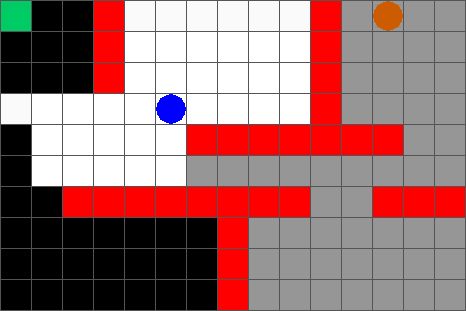
\includegraphics[scale=0.17]{figs/search_t2.png}\hspace{.5cm}
		}
		\subfloat[$t_7$ \label{fig:search2}]{
			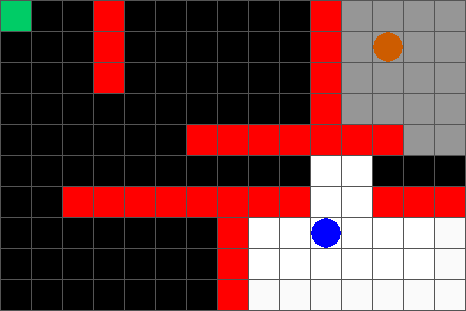
\includegraphics[scale=0.17]{figs/search_t3.png}\hspace{.5cm}
		}
		\subfloat[$t_9$ \label{fig:search3}]{
			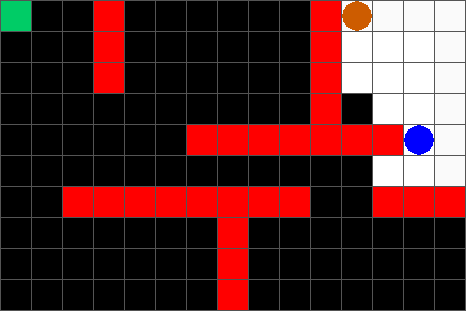
\includegraphics[scale=0.17]{figs/search_t4.png}\hspace{.5cm}
		}
	\end{minipage}
	\caption{The agent has to search for the target in order to lower its belief below the surveillance liveness specification.
	}
	\label{fig:search}
	
\end{figure}

In this example, an abstraction partition of size 7 was enough to guarantee the satisfaction surveillance specification.  For the purpose of comparison, we also solve the game with  an abstraction partition of size 12  to illustrate the change in belief growth. Figure \ref{fig:case1fineexp} shows the belief states growing much more slowly as the abstract belief states are smaller, and thus they more closely  approximate the true belief of the agent.
\begin{figure}
	\begin{minipage}{5.0cm}
		\centering
		\subfloat[$t_1$ \label{fig:casefine1t2}]{
			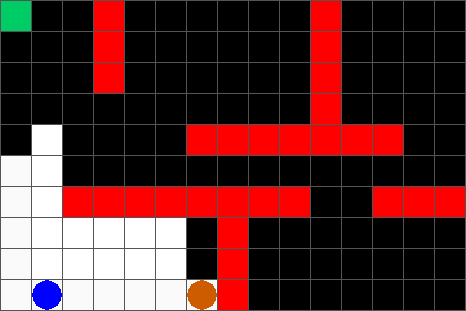
\includegraphics[scale=0.17]{figs/Liveness_t1.png}\hspace{.5cm}
		}
		\subfloat[$t_3$ \label{fig:case1finet3}]{
			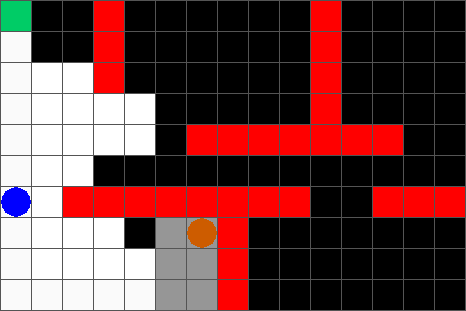
\includegraphics[scale=0.17]{figs/Liveness_fine_t11.png}\hspace{.5cm}
		}
		\subfloat[$t_4$ \label{fig:case1finet4}]{
			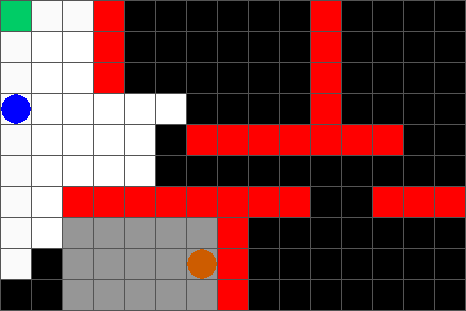
\includegraphics[scale=0.17]{figs/Liveness_fine_t2.png}\hspace{.5cm}
		}
	\end{minipage}
	\begin{minipage}{5.0cm}
		\centering
		\subfloat[$t_5$  \label{fig:case1finet5}]{
			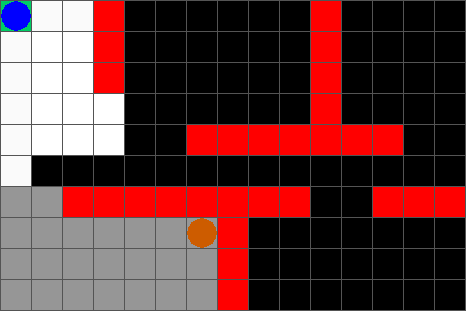
\includegraphics[scale=0.17]{figs/Liveness_fine_t3.png}\hspace{.5cm}
		}
		\subfloat[$t_6$ \label{fig:case1finet6}]{
			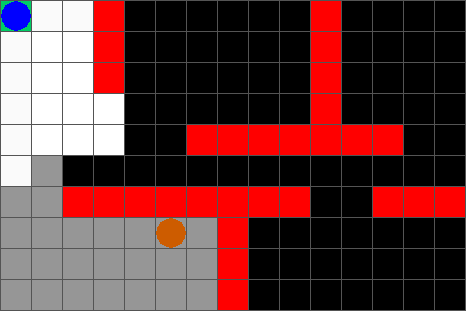
\includegraphics[scale=0.17]{figs/Liveness_fine_t4.png}\hspace{.5cm}
		}
		\subfloat[$t_7$ \label{fig:case1finet7}]{
			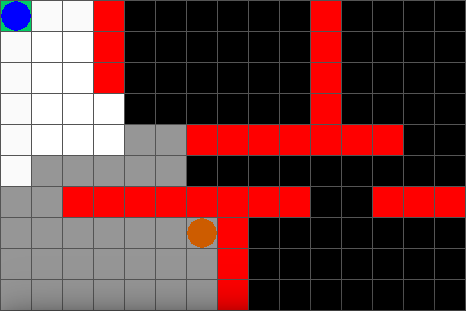
\includegraphics[scale=0.17]{figs/Liveness_t5.png}\hspace{.5cm}
		}
		
	\end{minipage}
	
	
	\caption{Evolution of the agent's belief about the target's location in a game  with an abstraction partition of size 12.
	}
	\label{fig:case1fineexp}
	
\end{figure}


The additional abstraction partitions result in a much larger game as the state space grows exponentially in the size of the abstraction partition. Table \ref{tab:exp1} compares the sizes of the corresponding abstract games, and the time it takes to synthesize a surveillance controller in each case.


\begin{table}[h!]
	\centering
	\begin{tabular}{c|c|c}
	Size of abstraction partition & Size of abstract game & Synthesis time \\ \hline \hline
		7 & 278 & 237s \\ 
		12 & 4346 & 810s \\ 
	\end{tabular}\caption{Comparison of synthesis times for the two cases} \label{tab:exp1}
\end{table}


A video simulation can be found at \url{http://goo.gl/YkFuxr}.

\subsection{Safety surveillance specification + task specification}
\begin{figure}
\centering
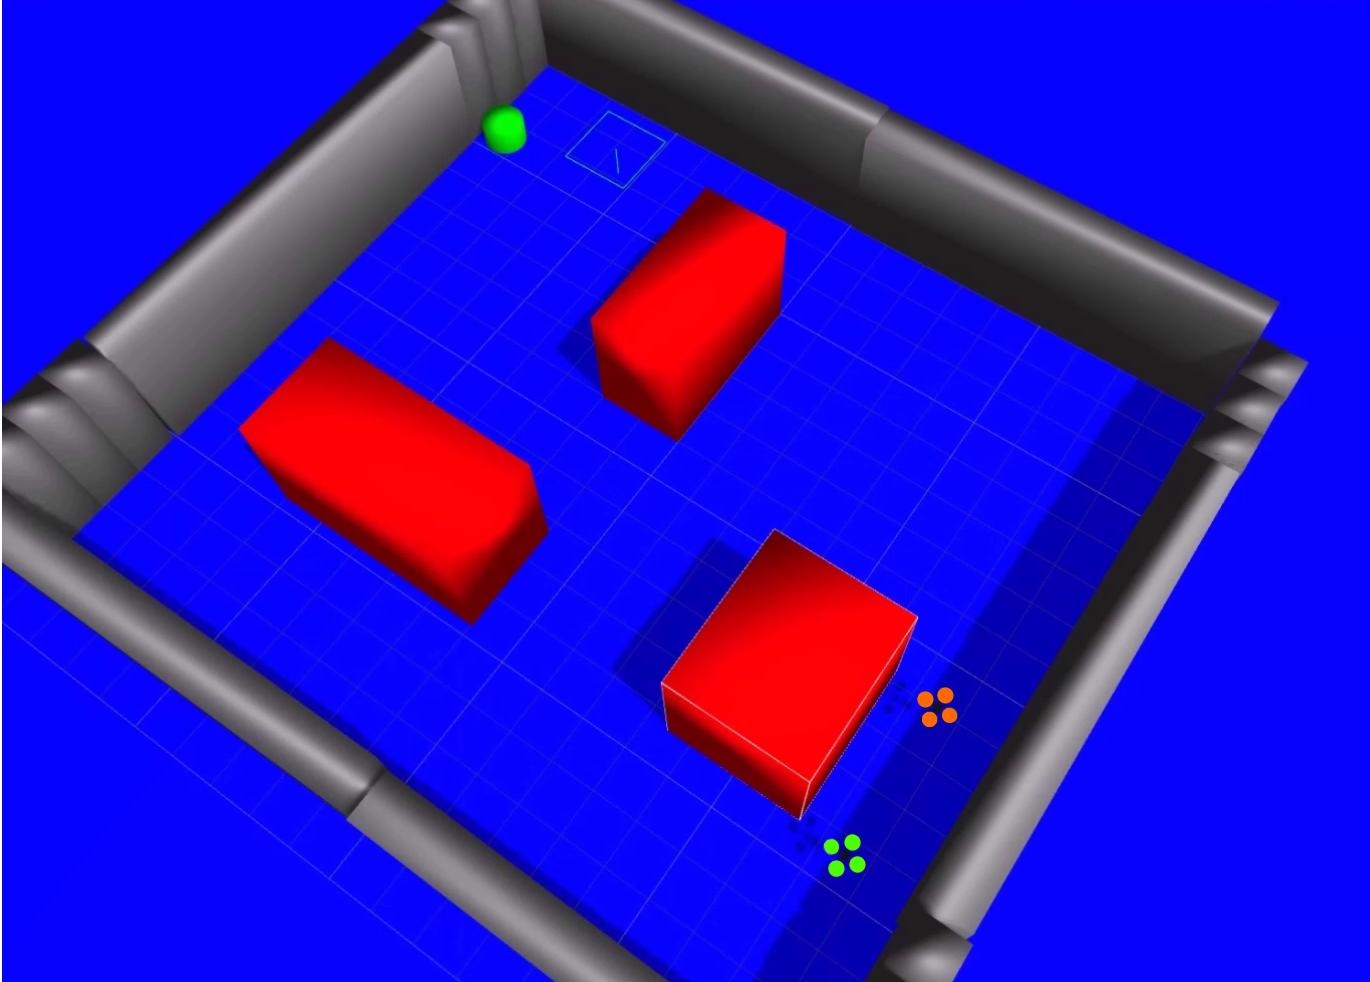
\includegraphics[scale=0.13]{figs/ROS_fig.png}\caption{A Gazebo environment where the red blocks are obstacles that the drones cannot see past. The green drone is the agent and the orange drone is the target.}\label{fig:case2}
\vspace{-.5cm}
\end{figure}
Figure~\ref{fig:case2} depicts an environment created in \emph{Gazebo} where the red blocks model buildings. The drone is given full line of sight vision - it can detect the target if there is no obstacle in the way. 
In this setting, we enforce the safety surveillance objective $\square p_{30}$ (the belief size should never exceed 30) in addition to infinitely often reaching the green cell. The formal specification is $\LTLglobally\LTLfinally p_{30} \wedge \LTLglobally\LTLfinally \mathit{goal}$. Additionally, the target itself is trying to reach the goal cell infinitely often as well, which is known to the agent.

We used an abstraction generated by a partition of size 6, which was sufficiently precise to compute a surveillance strategy in 210 s. Again, note that the precise belief-set game would have in the order of $2^{200}$ states.
 
We simulated the environment and the synthesized surveillance strategy for the agent in Gazebo and ROS. A video of the simulation can be found at \url{http://goo.gl/LyC1gQ}. This simulation presents a qualitative difference in behaviour compared to the previous example. There, in the case of liveness surveillance, the agent had more leeway to completely lose the target in order to reach its goal location, even though the requirement of reducing the size of the belief to $1$ is quite strict. Here, on the other hand, the safety surveillance objective, even with a large threshold of $30$, forces the agent to follow the target more closely, in order to prevent its belief from getting too large. The synthesis algorithm thus provides the ability to obtain qualitatively different behaviour as necessary for specific applications by combining different objectives. 

%\Suda{Not sure if we should keep this next part}
\subsection{Discussion}
The difference in the behaviour in the case studies highlights the different use cases of the surveillance objectives. Depending on the domain, the user can specify a combination of safety and liveness specification to tune the behaviour of the agent. In a critical surveillance situation (typical in defense or security situations), the safety specification will guarantee to the user that the belief will never grow too large. However, in less critical situations (such as luggage carrying robots in airports), the robot has more flexibility in allowing the belief to grow as long as it can guarantee its reduction in the future. 